\documentclass[a4paper]{article}

\usepackage{graphicx}

\usepackage{hyperref}
\usepackage[utf8]{inputenc}
\usepackage[T1]{fontenc}
\usepackage[serbian]{babel}
\usepackage{xcolor}
\usepackage{dirtytalk}
\usepackage{float}
\usepackage{subcaption}
\title{Uputstvo za upotrebu i sklapanje elektronike za Integra wall}
\author{Nemanja Filipovic, \href{mailto:nemanja.filipovic96@gmail.com}{nemanja.filipovic96@gmail.com}}
\def\bitno#1{\textbf{\textcolor{red}{Bitno:}} \textit{#1}}
\begin{document}
	\maketitle
	
	\section{Povezivanje komponenti}
	
	Elektronika za Integra wall se sastoji iz nekoliko odvojenih celina:
	\begin{enumerate}
		\item Raspberry pi sa monitorom 
		\item Plo\v ca sa senzorima (slika \ref{fig:sensors})
		\item LE diode i odgovaraju\' ce napajanje sa otpornicima
		\item Senzor pra\v sine sa modulom za komunikaciju
		\item Napajanje za Raspberry pi sa monitorom (u trenutnoj iteraciji, USB punja\v c)
	\end{enumerate}
	
	\begin{figure}[H]
		\centering
		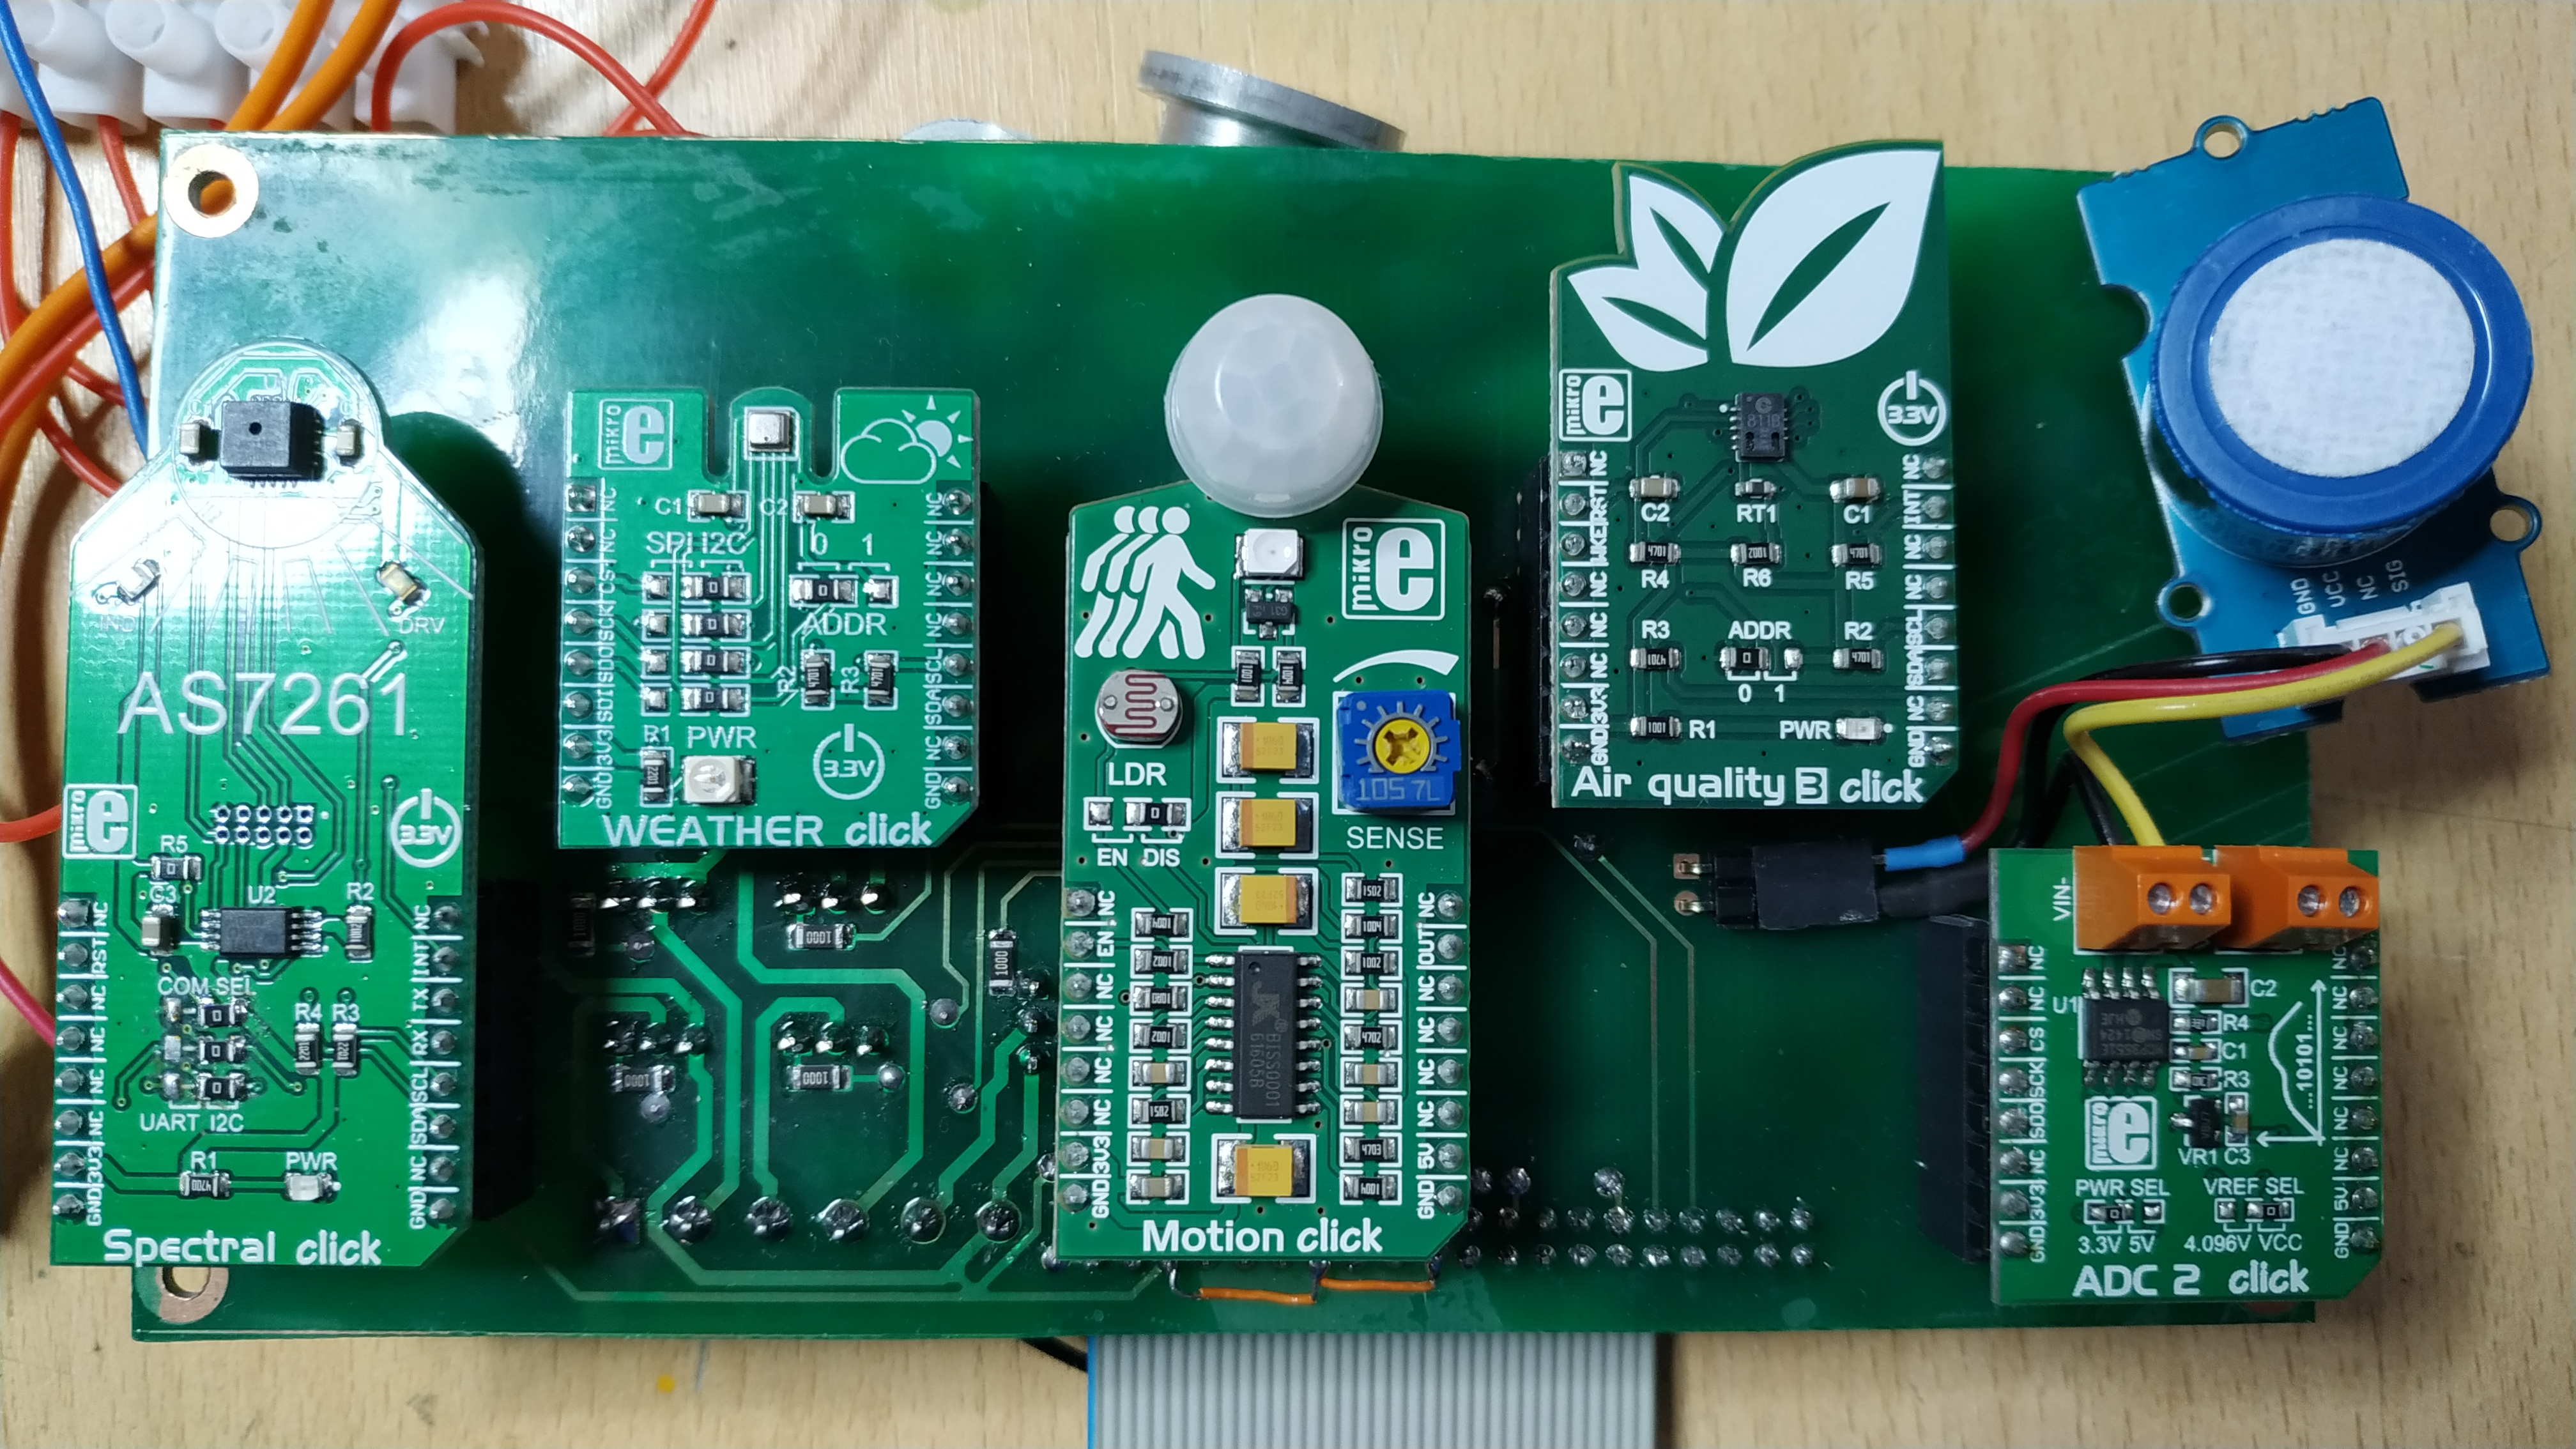
\includegraphics[width=0.6\textwidth]{graphics/sensorBrd.jpg}
		\caption{Plo\v ca sa senzorima}
		\label{fig:sensors}
	\end{figure}
	
	Raspberry pi je trajno pri\v cvr\v s\' cen na monitor pomo\' cu odstojnika koji su fabri\v cki dostavljeni.
	Elektri\v cna konekcija izme\dj u ta dva modula je ostvarena pomo\' cu pljosnatog kabla bele boje. 
	\bitno{Trakasti kabl za povezivanje sa monitorom je izuzetno lako pokriviti tako da se provodnici slome.
	Obratiti posebnu pa\v znju na to}. Raspberry pi i monitor ne treba odvajati prilikom instalacije.
	
	Elektri\v cna konekcija izme\dj u plo\v ce sa senzorima i Raspberry pi-a ostvarena je pomo\' cu sivog
	traka kabla sa 34 provodnika. Konektori na kraju kabla imaju 40 pinova. Predvi\dj eno je da se tokom 
	ugradnje ovaj kabl otka\v ci sa konektora na oba kraja. Ponovnu konekciju je potrebno ostvariti na na\v cin
	prikazan na slici \ref{fig:overall}. Kraj kabla na kome je ispisano \say{PI} treba da bude bli\v zi
	Raspberry pi-u, a kraj sa ispisanim \say{S} treba da bude uz senzorsku plo\v cu.
	 \bitno{Ukoliko se konektori pogre\v sno orijenti\v su, gotovo je 
	zagarantovana destrukcija Raspberry pi-a i/ili elektronike na plo\v ci sa senzorima. Obratiti
	posebnu pa\v znju pri povezivanju}.
	
	\begin{figure}[H]
		\centering
		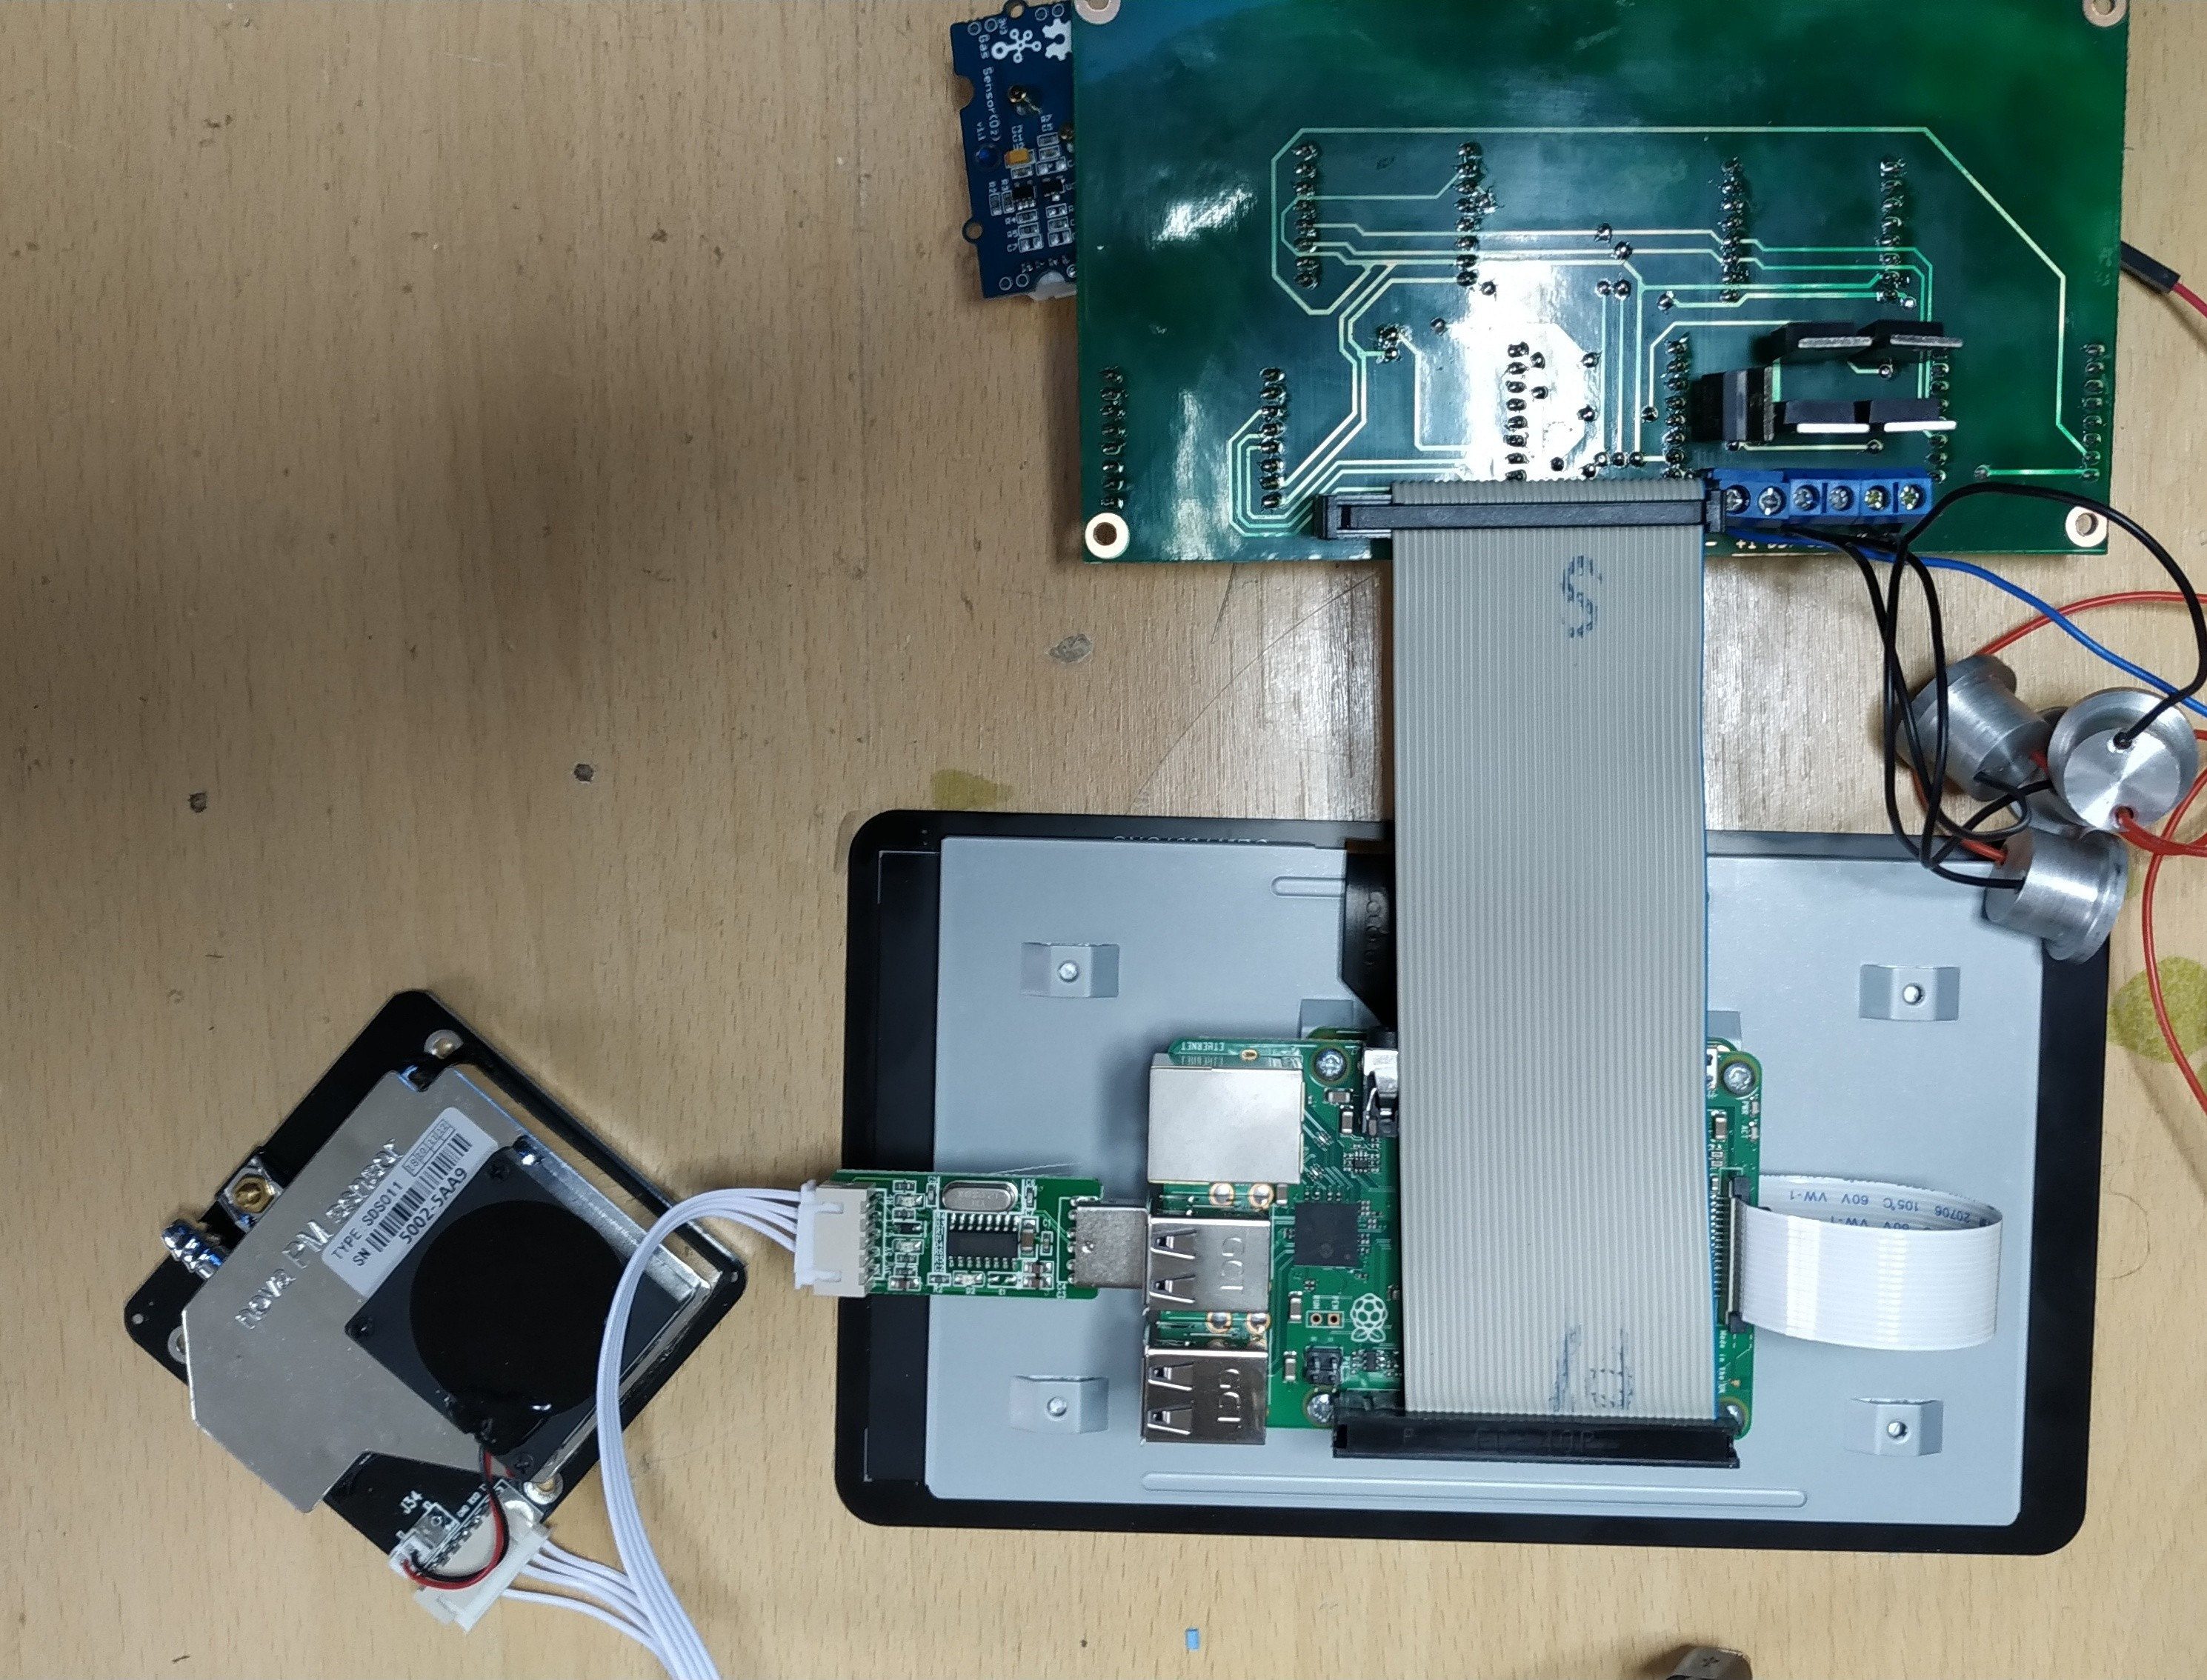
\includegraphics[width=0.6\textwidth]{graphics/overall.jpg}
		\caption{Povezivanje elektronike}
		\label{fig:overall}
	\end{figure}
	
	Senzor pra\v sine se povezuje putem USB konektora na sistem. Va\v zno je da senzor bude povezan 
	na ta\v cno odre\dj eni port kako bi program mogao uspe\v sno da ostvari komunikaciju. Pozicija porta
	prikazana je na slici \ref{fig:usb}.
	
	\begin{figure}[H]
		\centering
		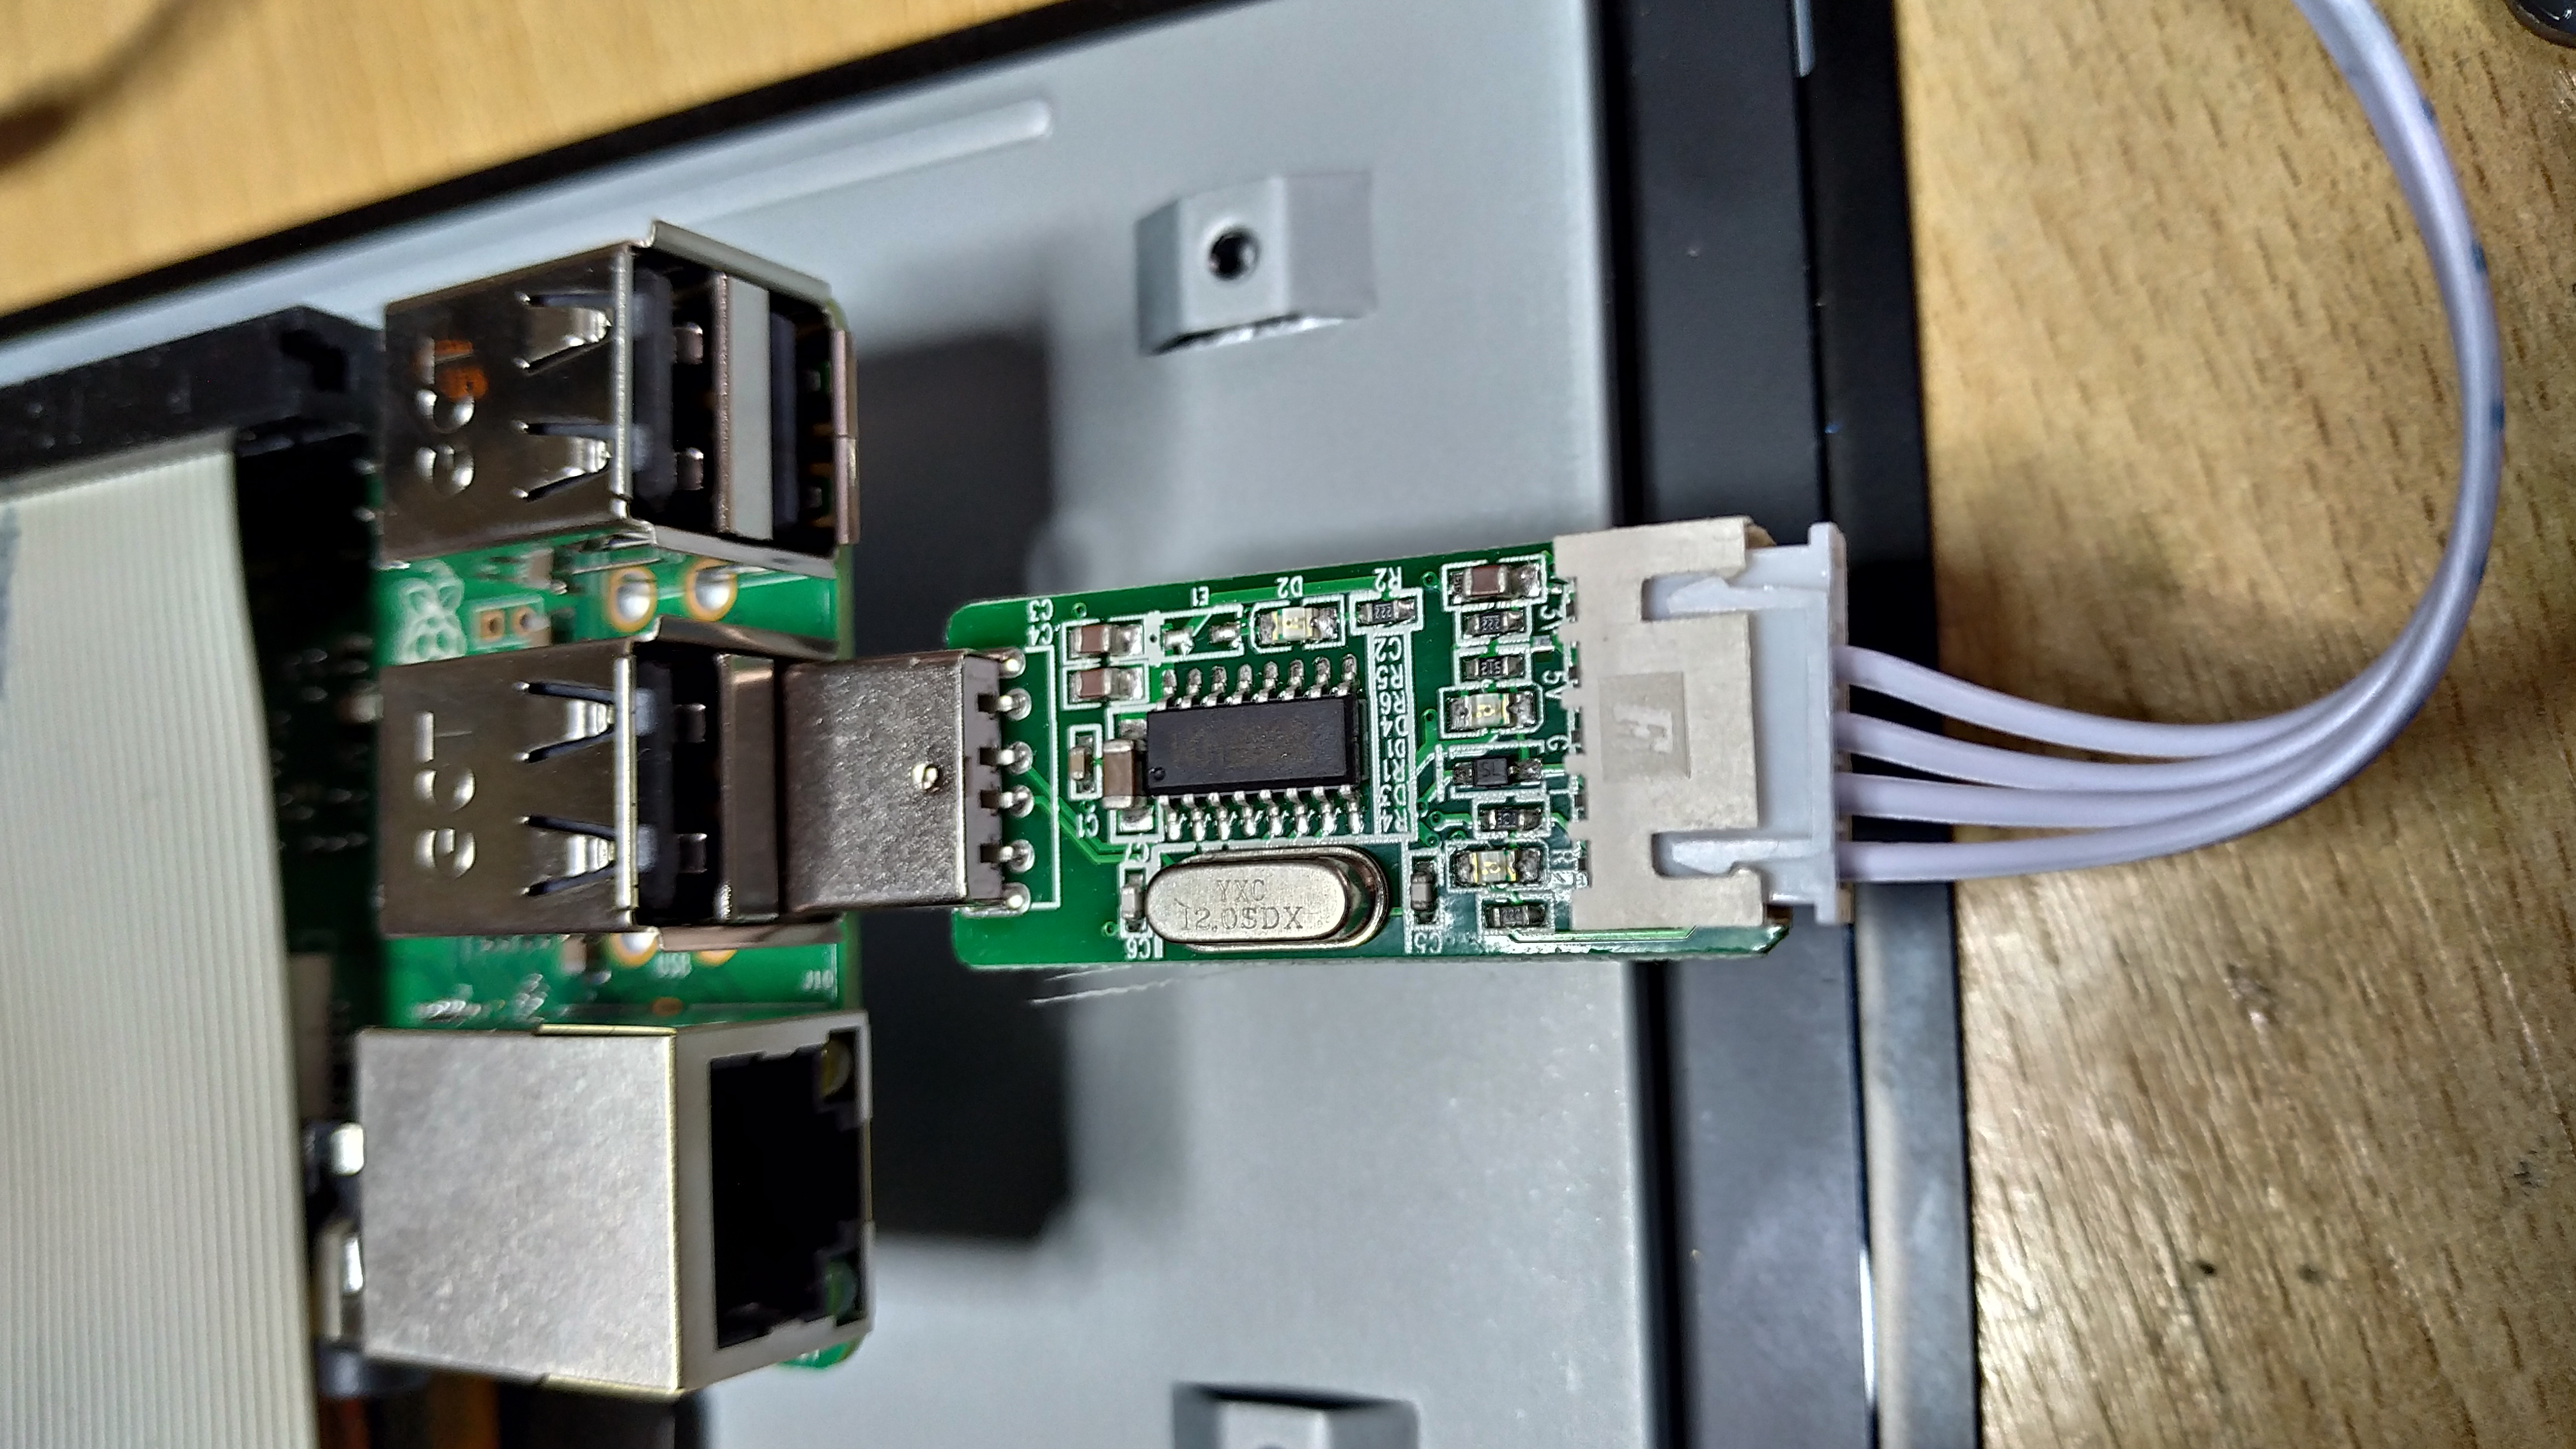
\includegraphics[width=0.6\textwidth]{graphics/dustConection.jpg}
		\caption{Povezivanje senzora pra\v sine}
		\label{fig:usb}
	\end{figure}
	
	Konekcija sa LE diodama se ostvaruje preko print kleme (slika \ref{fig:LED}). 
	\begin{figure}[H]
		\centering
		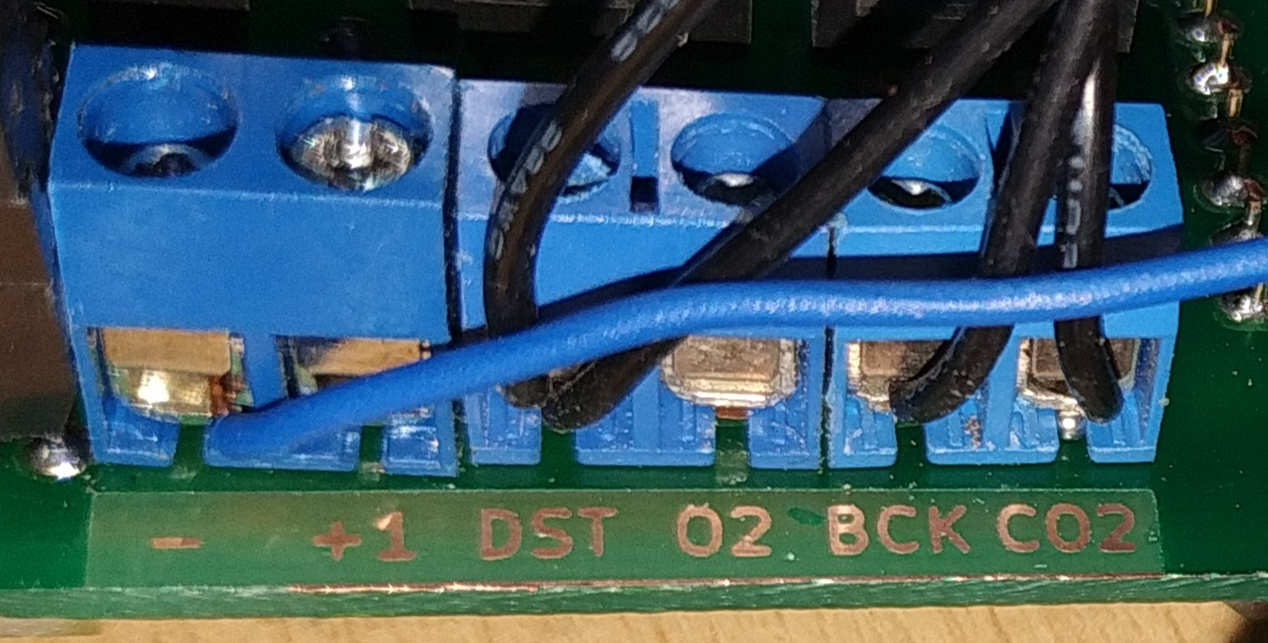
\includegraphics[width=0.6\textwidth]{graphics/LEDs.jpg}
		\caption{Povezivanje LE dioda}
		\label{fig:LED}		
	\end{figure}		
	Svaka kontrolisana LED 
	pozicija ima svoj kanal. Na plo\v cu se dovode negativni krajevi LED svetiljki i povezuju se sa 
	odgovaraju\' ce ozna\v cenim konekcijama. Kanali imaju kapacitet do 1.2A.
	
	Oznake kanala zna\v ce slede\' ce:
	\begin{enumerate}
		\item \say{\texttt{-}} - Negativan kraj napajanja za LE diode
		\item \say{\texttt{+1}} - Rezervni kanal za slu\v caj pro\v sirivanja funkcionalnosti
		\item \say{\texttt{DST}} - Kanal indikatora za senzor pra\v sine
		\item \say{\texttt{O2}} - Kanal indikatora za senzor kiseonika
		\item \say{\texttt{BCK}} - Kanal LED trake povezane sa senzorom pokreta i osvetljenja
		\item \say{\texttt{CO2}} - Kanal indikatora za senzor ugljen-dioksida
	\end{enumerate}
	
	Povezivanje napajanja se vr\v si putem dva mikro USB kabla (kao za punjenje telefona). Jedan kabl napaja
	monitor, dok drugi kabl napaja Raspberry pi. Na slici \ref{fig:power} je prikazan na\v cin njihovog 	
	povezivanja.
	\begin{figure}[H]
		\centering
		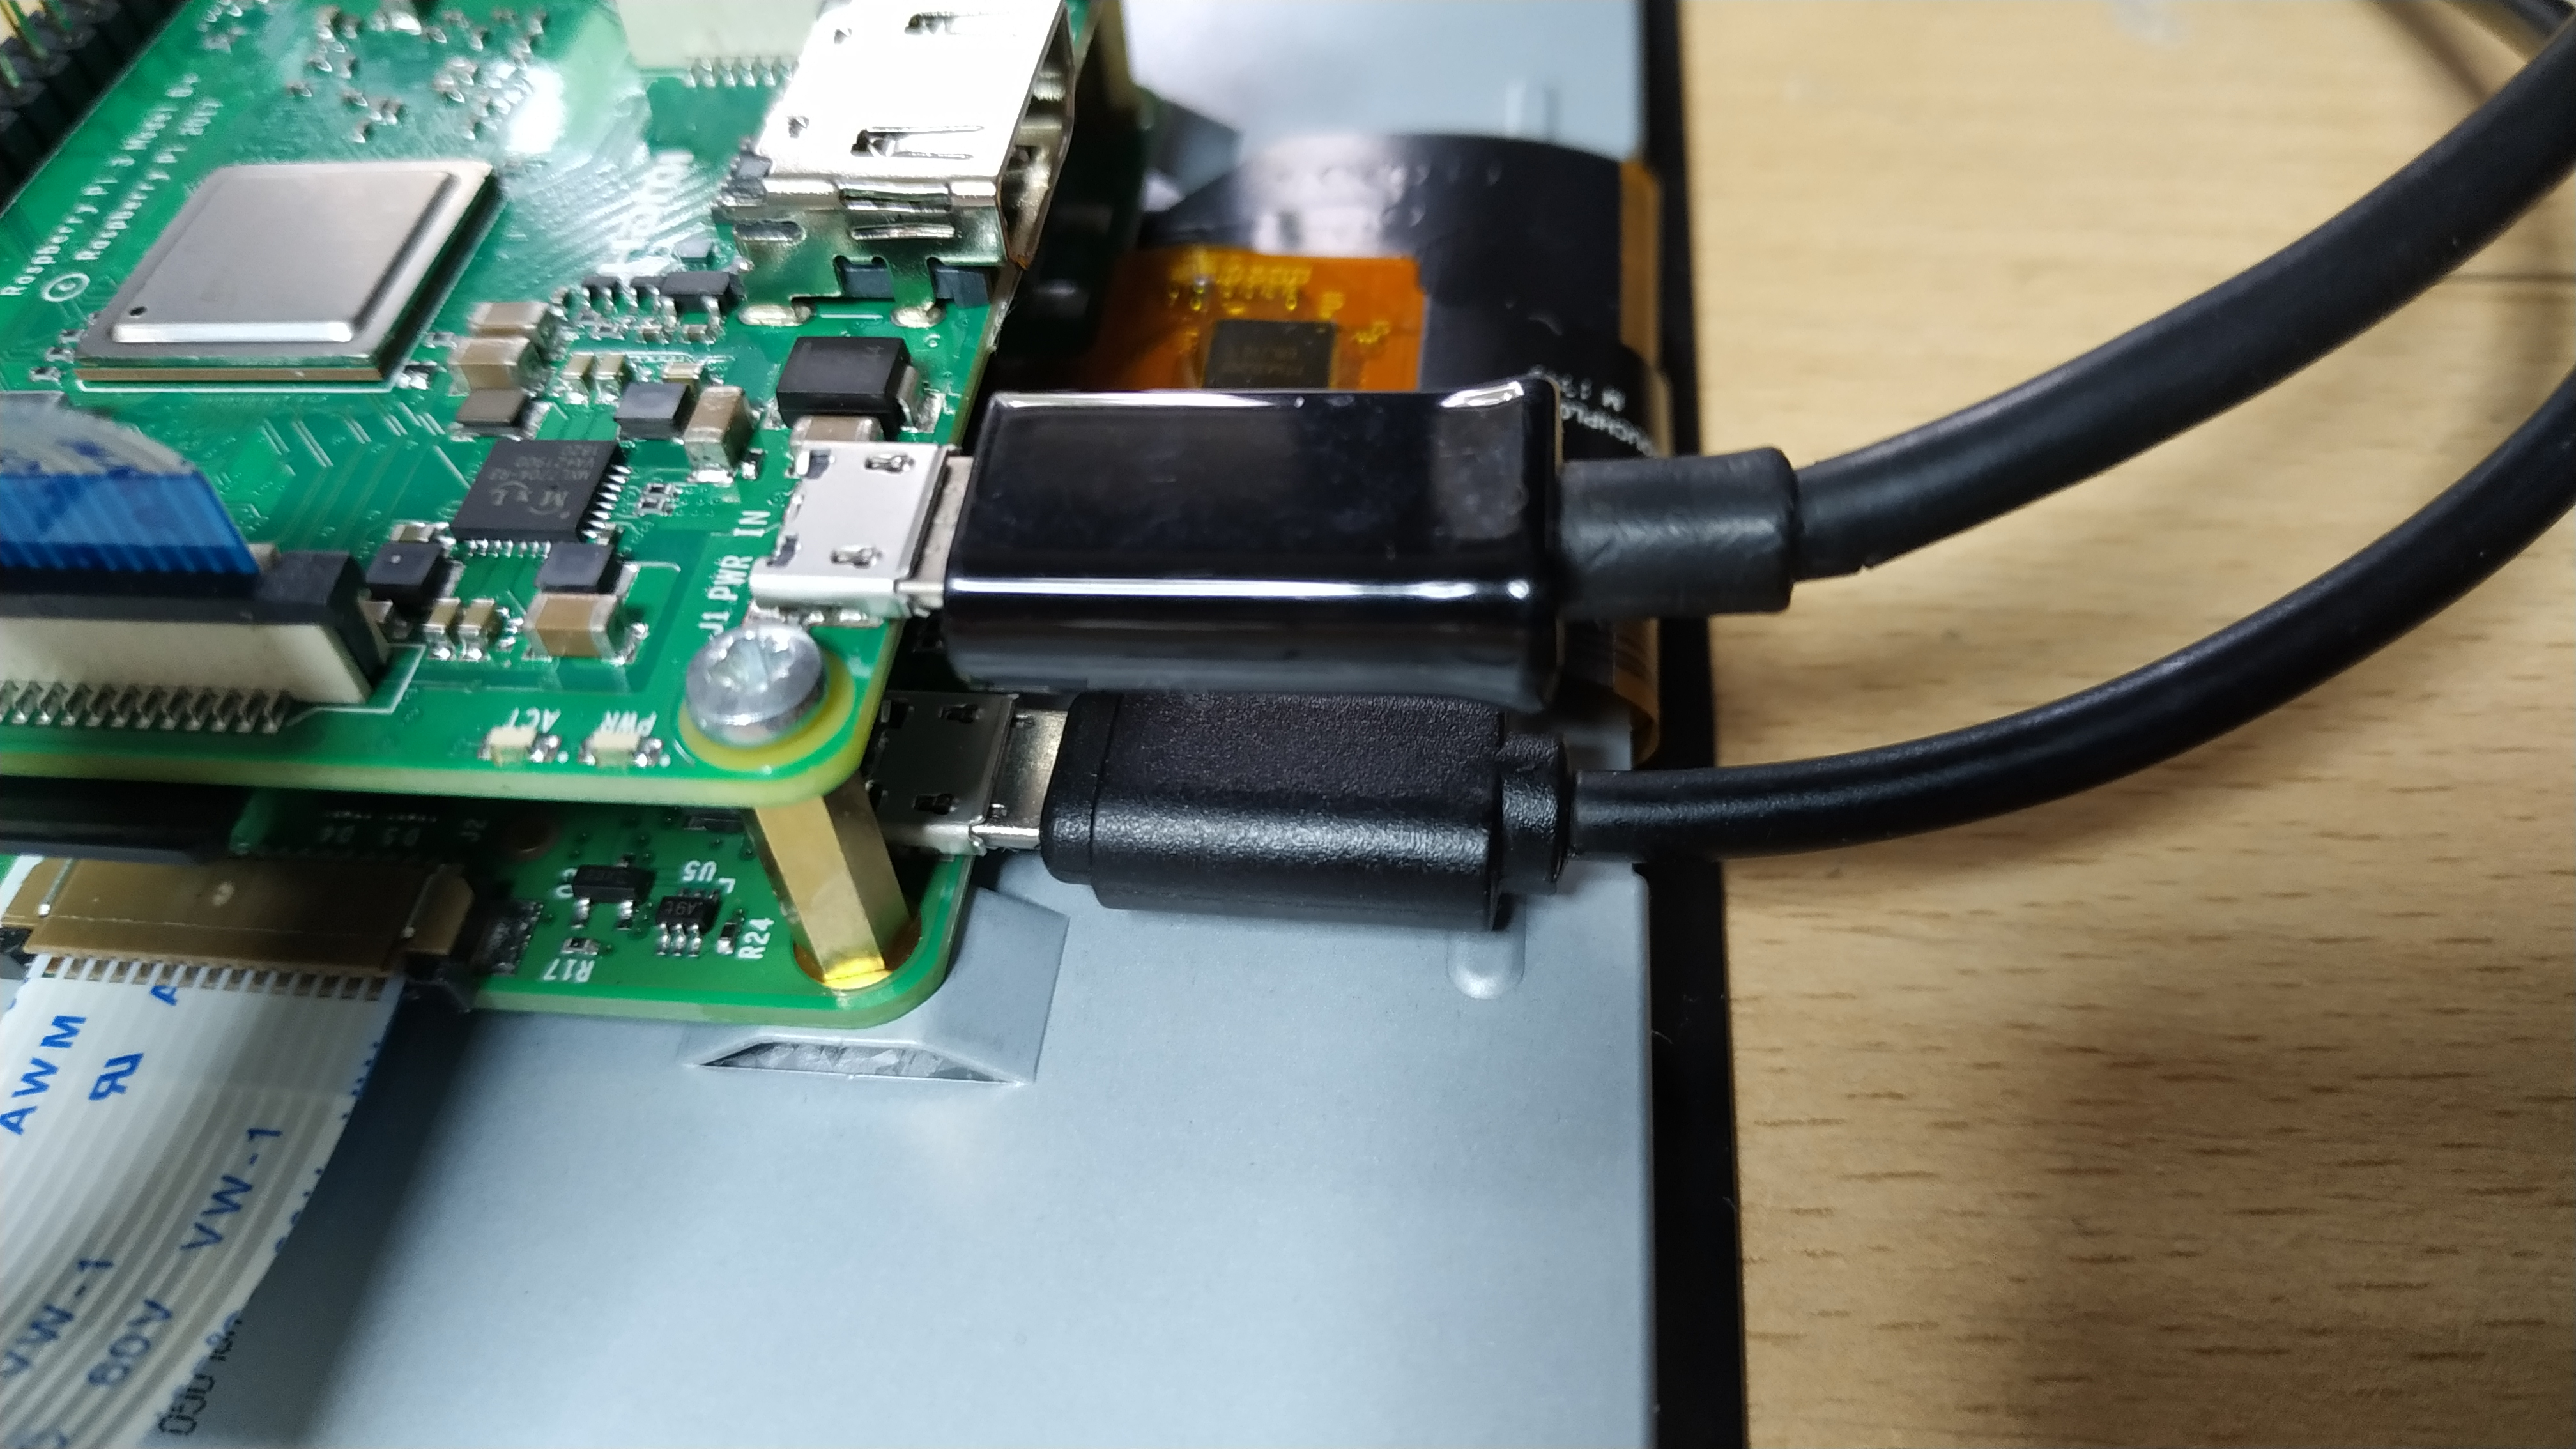
\includegraphics[width=0.6\textwidth]{graphics/USB.jpg}
		\caption{Povezivanje napajanja}
		\label{fig:power}		
	\end{figure}	
	
	Za izvor napajanja je izabran punja\v c za telefon, \href{https://www.gigatron.rs/punjaci_za_mobilne_telefone/acme_ch205_wall_charger_-_a504597-173419?recommender_box_placement=productpage_similar&recommender_box=quarticon}{Acme CH205}. Njegove specifikacije
	su prikazane na slici \ref{fig:charger}. \bitno{Punja\v c mora da ostvari radnu struju od bar 2.4A na 5V.
	Potrebno je koristiti \v sto kra\' ce USB kablove}.
	\begin{figure}[H]
		\centering
		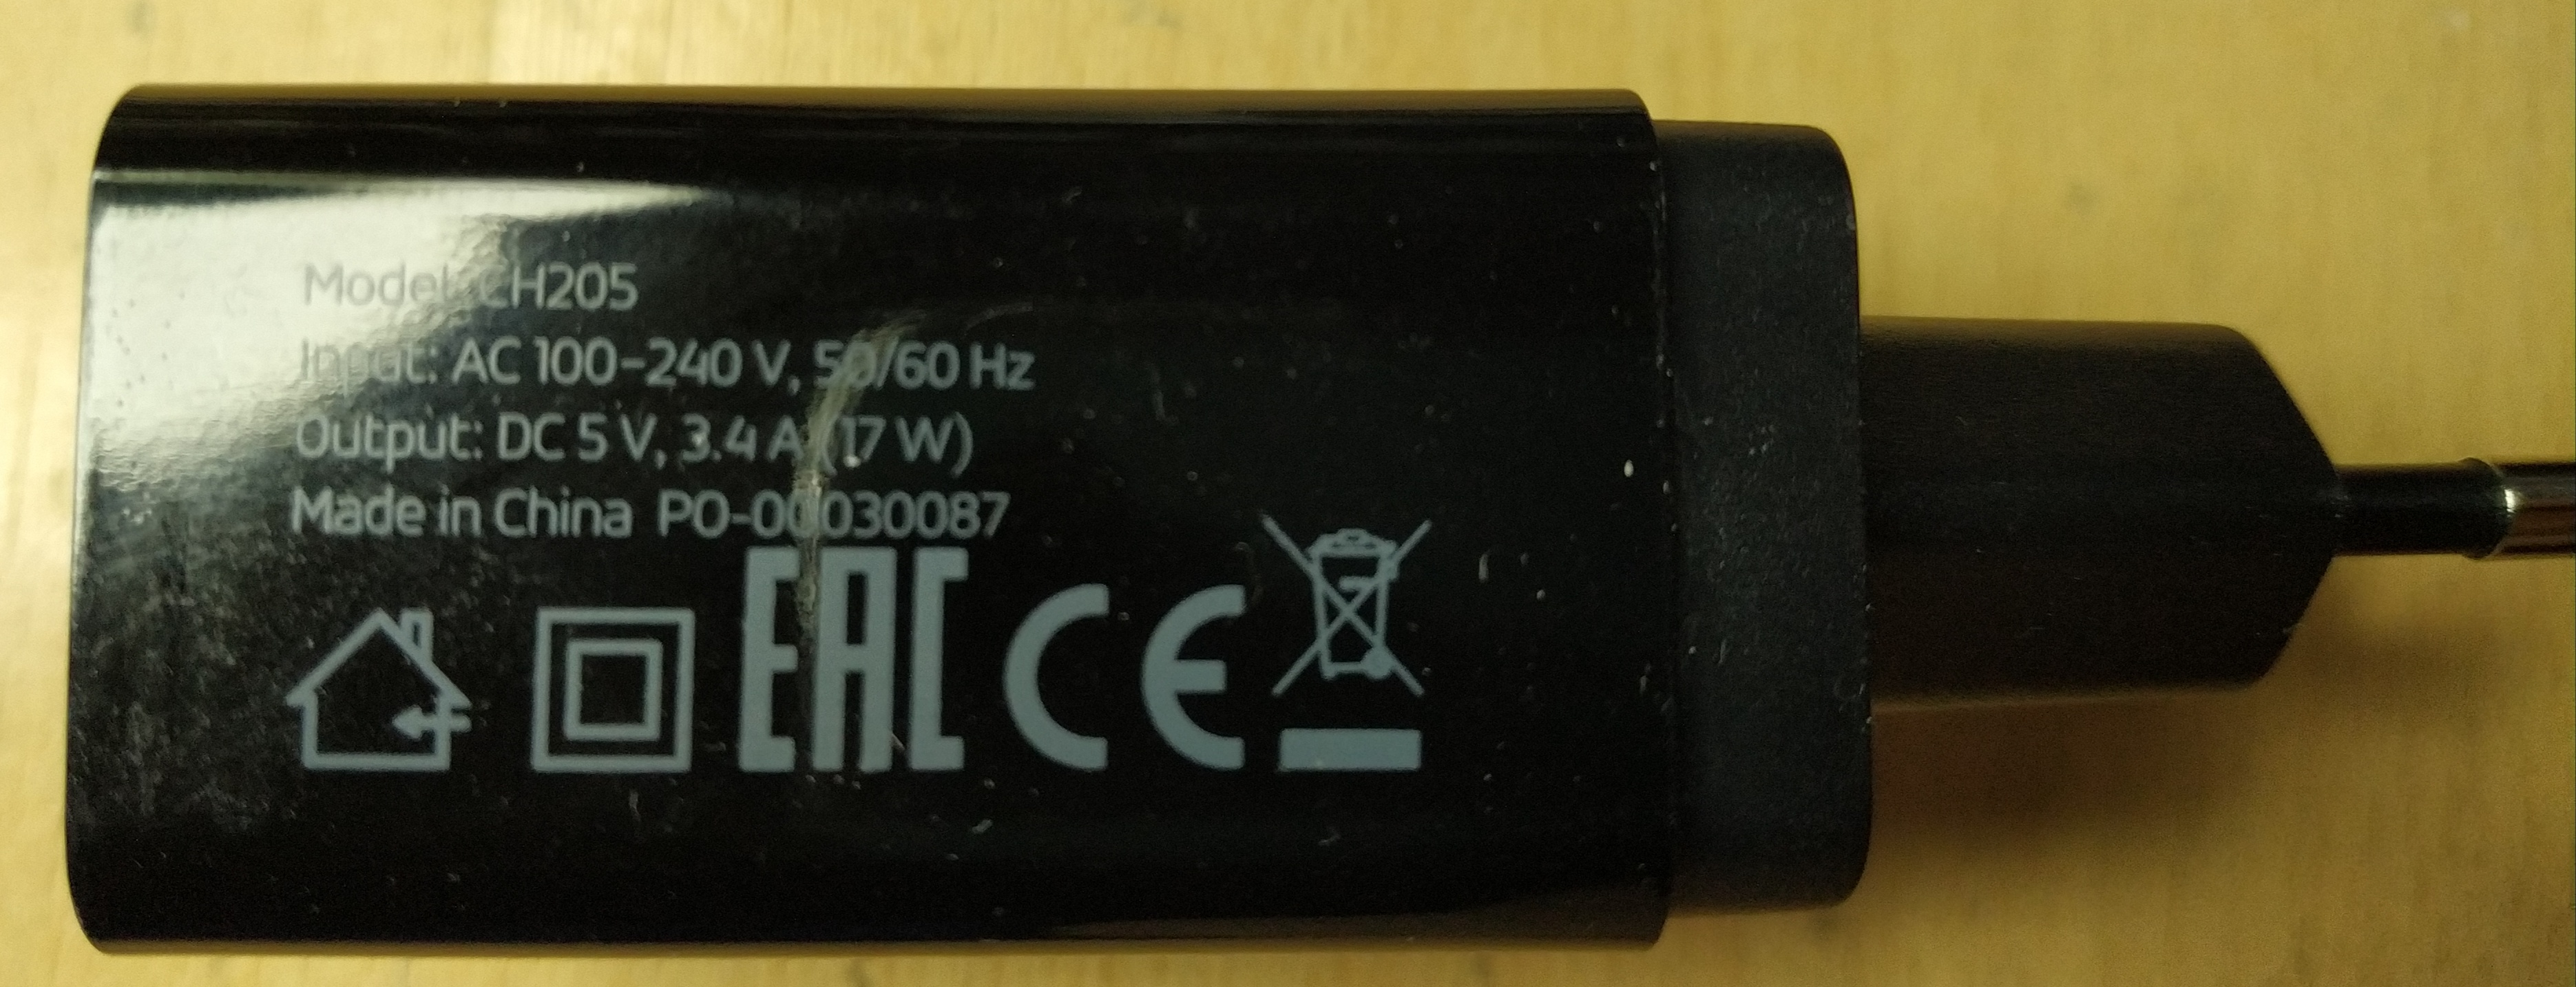
\includegraphics[width=0.6\textwidth]{graphics/charger.jpg}
		\caption{Kori\v s\' ceni punja\v c}
		\label{fig:charger}	
	\end{figure}
	\section{Povezivanje ure\dj aja na Internet}
	
	Za povezivanje Raspberry pi-a na lokalnu mre\v zu ili internet, potrebno je obezbediti \v zi\v cnu
	(standardni ethernet priklju\v cak) ili be\v zi\v cnu (WiFi, 2.4GHz) konekciju. Za \v zi\v cnu konekciju
	nije potrebna konfiguracija sa strane ure\dj aja. Ukoliko je potreban pristup ure\dj aju iz lokalne 
	mre\v ze, neophodno je izvr\v siti pode\v savanja DHCP servera tako da se dodeljuje stati\v cka IP
	adresa. Pode\v savanje se vr\v si prema korisni\v ckom uputstvu za ruter.
	
	U slu\v caju da se konekcija vr\v si putem WiFi-a, neophodno je izvr\v siti pode\v savanje kredencijala.
	Ovo je najjednostavnije u\v ciniti na drugom PC ra\v cunaru. Potrebno je izvaditi mikroSD karticu
	(koja je pozicionirana direktno ispod belog traka kabla koji je povezan sa displejem). Na njoj se nalazi 
	drajv pod nazivom \say{\texttt{boot}}. Pode\v savanja se izvode u fajlu \texttt{wpa\_supplicant.conf}. 
	Taj fajl otvoriti pomo\' cu Notepad-a (ili sli\v cnog programa) i izvr\v siti konfiguraciju za datu WiFi 
	mre\v zu. Deo fajla ima sadr\v zaj slede\' ceg formata:
	\begin{verbatim}
network={
    ssid="<SSID>"
    psk="<Sifra>"
}
	\end{verbatim}
	Zameniti \texttt{<SSID>} i \texttt{Sifra} odgovaraju\' cim vrednostima (zadr\v zavaju\' ci znake navoda).
	U slu\v caju da postoji vi\v se mre\v za, mogu\' ce je kopirati ceo prikazani odeljak vi\v se puta, \v cime
	se omogu\' cava da se ure\dj aj automatski konektuje na bilo koju od prisutnih mre\v za.
	
	\bitno{Ure\dj aj nema sat realnog vremena sa bekap baterijom, te pri svakom nestanku napajanja
	ure\dj aj gubi ta\v cno vreme i datum. Ta\v cno vreme se automatski pode\v sava periodi\v cno ukoliko je
	prisutna konekcija sa Internetom. Ukoliko te konekcije nema po uklju\v cenju, vremena upisana u log fajlove
	ne\' ce biti validna.}
	
	\section{Udaljen pristup merenjima i log fajlovima}
	
	Nakon povezivanja na lokalnu mre\v zu, ure\dj aju je dodeljena lokalna IP adresa (oblika na primer
	\texttt{192.168.0.24}). Ta lokalna IP adresa \' ce biti kori\v s\' cena za dalji pristup. U daljem tekstu
	\' ce biti navo\dj ena u obliku \texttt{<ADRESA>}. Za prikaz merenja kao i na displeju, potrebno je
	putem web pretra\v ziva\v ca pristupiti strani \texttt{<ADRESA>:5000}. 
	
	Ure\dj aj omogu\' cava i logovanje merenja na regularnim intervalima. Log fajlovi se \v cuvaju u memoriji
	i nakon nestanka napajanja i mogu\' ce je njihovo preuzimanje kori\v s\' cenjem web interfejsa. 
	Za pristup log fajlovima, potrebno je pristupiti strani \texttt{<ADRESA>:5000/logs} (slika \ref{fig:logs}).
	\begin{figure}[H]
		\centering
		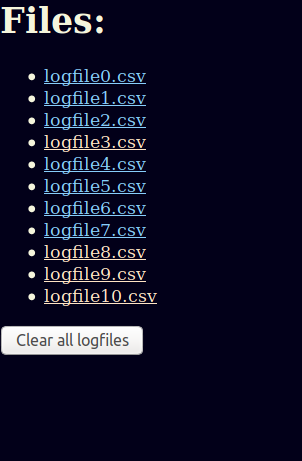
\includegraphics[width=0.3\textwidth]{graphics/logs.png}
		\caption{Izgled strane za pristup log fajlovima}
		\label{fig:logs}		
	\end{figure}	
	
	Pri svakom 
	uklju\v cenju se formira novi log fajl. Fajlovi su numerisani tako da najve\' ci indeks ozna\v cava 
	najnoviji fajl. Klikom na odgovaraju\' ci link, mo\v ze se preuzeti \texttt{.csv} fajl u kom se nalaze
	merenja. Nakon preuzimanja svih fajlova, omogu\' ceno je njihovo brisanje, kliko na dugme \say{Clear
	all logfiles}. Sajt \' ce zatim zahtevati od korisnika da potvrdi naredbu, a onda \' ce dobiti potvrdu
	o brisanju uz naveden broj obrisanih fajlova.
\end{document} 
